
\documentclass{beamer}

\useoutertheme[height=0.1\paperheight,width=0.1\paperwidth,hideothersubsections]{sidebar}
\usecolortheme{whale}
\usecolortheme{orchid}

\useinnertheme[shadow]{rounded}
\setbeamercolor{title page}{fg=blue!70,bg=blue}
\setbeamercolor{logo}{bg=blue!60}
\setbeamercolor{frametitle}{fg=black,bg=blue!60}
%\setbeamercolor{section in sidebar}{fg=red}
\setbeamercolor{block title}{bg=blue!28!white,fg=blue}
\setbeamercolor{block body}{bg=red!15!white}
\setbeamercolor{sidebar}{bg=blue!70}

\setbeamertemplate{background canvas}[vertical shading][bottom=white,top=blue!25]
\usefonttheme{serif}
\setbeamertemplate{navigation symbols}{}
\usepackage{tikz}
\usepackage{CJKutf8}
\usetikzlibrary{positioning}
\usetikzlibrary{calc}
\usetikzlibrary{trees}
%\usepackage{subfigure}
\usepackage{xmpmulti}
\usepackage{colortbl,dcolumn}
\graphicspath{{November/}}
\DeclareGraphicsRule{*}{mps}{*}{}

\logo{\includegraphics[width=0.1\paperwidth]{huoqiang.jpg}}
\renewcommand{\raggedright}{\leftskip=0pt \rightskip=0pt plus 0cm}
\raggedright
\def\hilite<#1>{\temporal<#1>{\color{blue!35}}{\color{magenta}}{\color{blue!75}}}

\newcolumntype{H}{>{\columncolor{blue!20}}c!{\vrule}}
\newcolumntype{H}{>{\columncolor{blue!20}}c}
\newcommand{\upcite}[1]{\textsuperscript{\cite{#1}}}
\bibliographystyle{plain}
\newcommand{\yihao}{\fontsize{30pt}{\baselineskip}\selectfont}
\newcommand{\sihao}{\fontsize{14pt}{\baselineskip}\selectfont}
\newcommand{\xiaosihao}{\fontsize{12pt}{\baselineskip}\selectfont}
\newcommand{\wuhao}{\fontsize{10.5pt}{\baselineskip}\selectfont}  
\newcommand{\xiaowuhao}{\fontsize{9pt}{\baselineskip}\selectfont} 
\newcommand{\liuhao}{\fontsize{7.875pt}{\baselineskip}\selectfont}
\newcommand{\qihao}{\fontsize{5.25pt}{\baselineskip}\selectfont}
\newcommand{\ThankYouPage}{
  \begin{frame}
    \yihao \centering \textcolor{blue}
    {Thank You!}
  \end{frame}
}

\begin{document}
\begin{CJK*}{UTF8}{gkai}
  \title{十一月工作总结}
  \author[\textcolor{black}{作者 朱海文}]{作者~~\textcolor{olive}{朱海文}}
  \institute{\textcolor{violet}{摩科特医疗器械有限公司}}
  \date{\today}
  \frame{\titlepage}
  %======================================================
  \section*{目录}
  \section{晶体上泄漏的光子}
  \frame{\frametitle{目录}\tableofcontents}
  %========================================
  \begin{frame}\frametitle{打到晶体表面的能量}
    \begin{figure}[ht]
      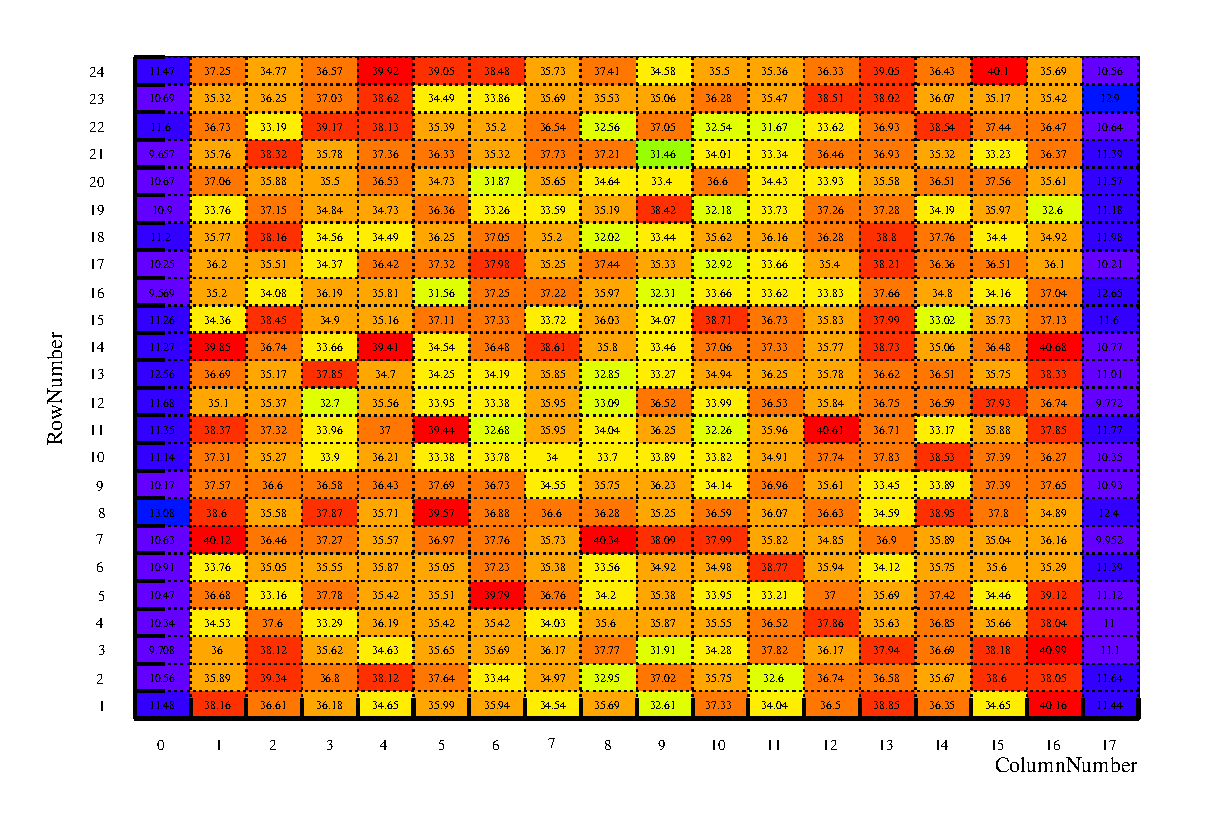
\includegraphics[width=\textwidth]{AttachCrystalEnergy.eps}
    \end{figure}
  \end{frame}
  %=========================
  \begin{frame}\frametitle{打到晶体表面的能量}
    \begin{minipage}[t]{0.2\textwidth}
      \liuhao
      从上图看,打到晶体表面的能量涨落比较明显,是由于事例数太少导致的,用单一能量的光子
      模拟,每块晶体上的光子数大于3000时涨落就比较小了。
    \end{minipage}
    \begin{minipage}[t]{0.8\textwidth}
      \vskip -0.5cm
      \begin{figure}[ht]
	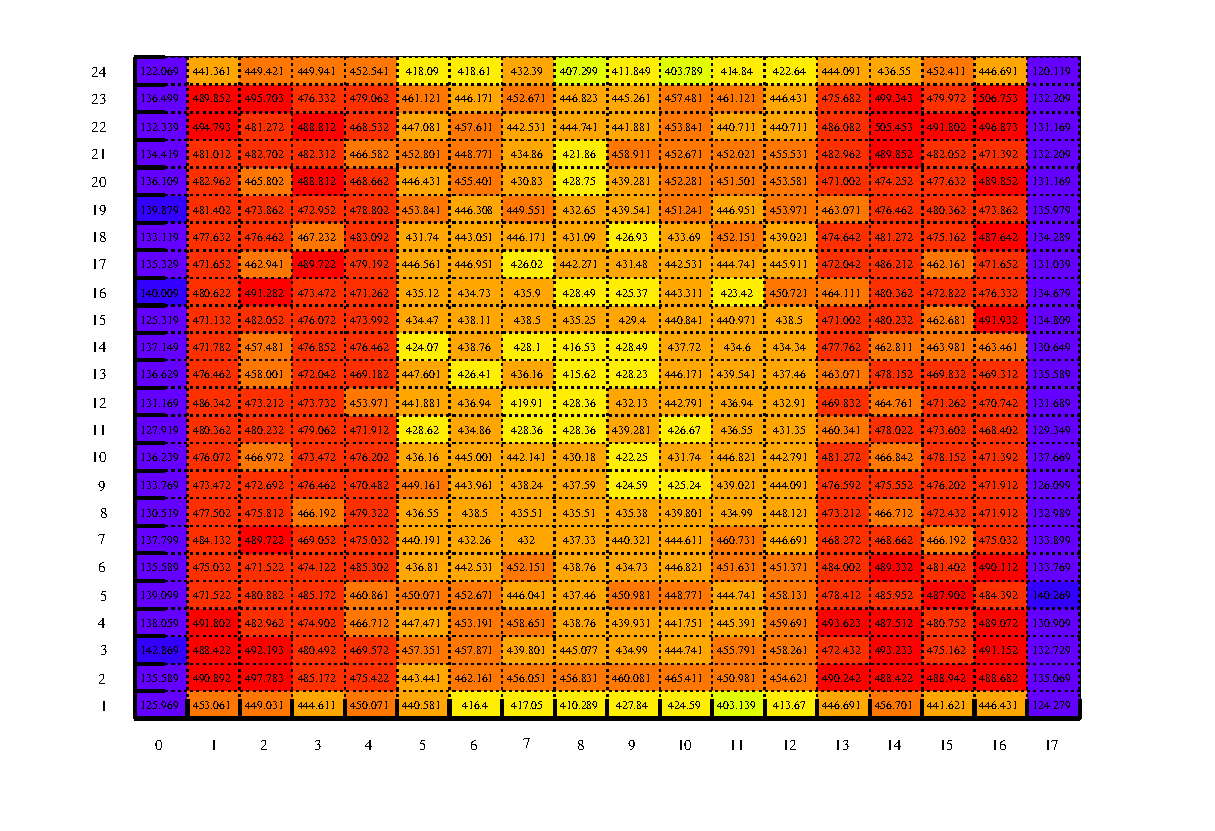
\includegraphics[width=0.78\textwidth]{SingleEnergyWaterDirectEnergy.eps}
	
	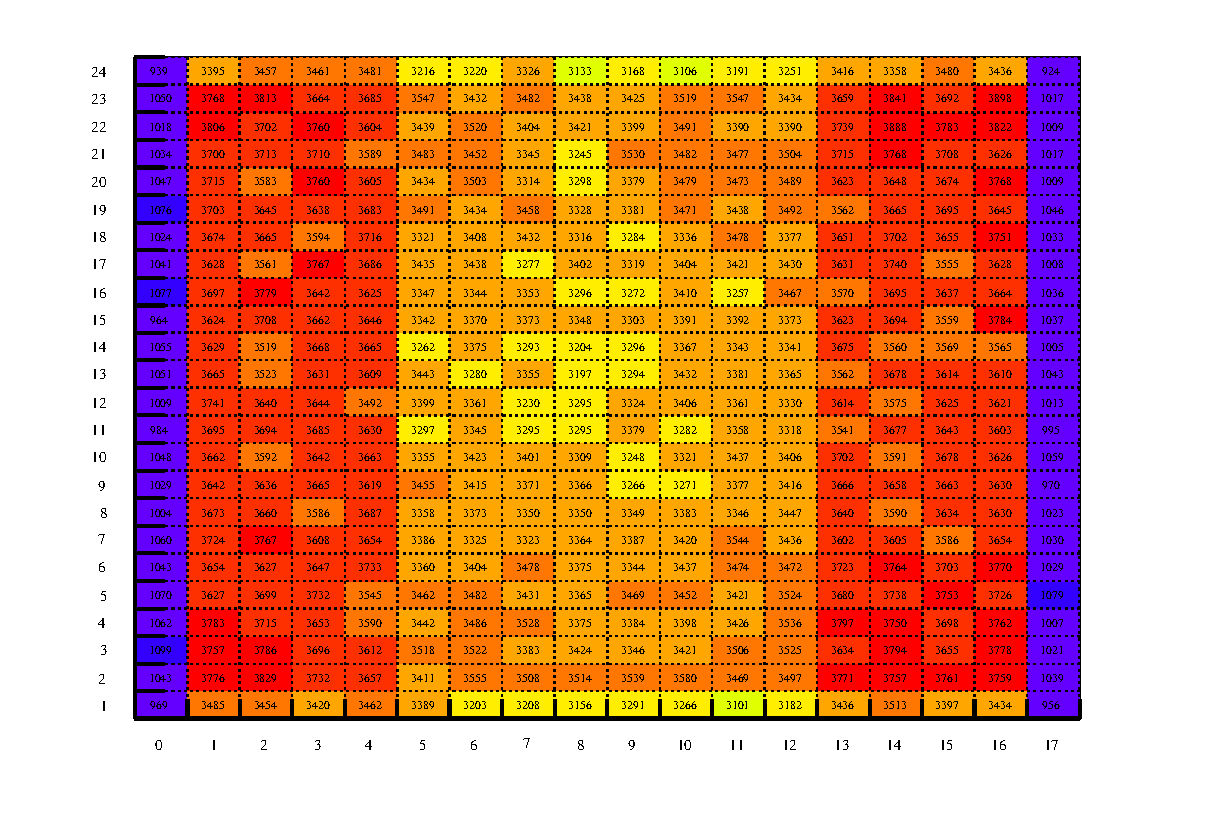
\includegraphics[width=0.78\textwidth]{SingleEnergyWaterDirectNumber.eps}
      \end{figure}
    \end{minipage}
  \end{frame}
  \begin{frame}\frametitle{统计每一块晶体上泄漏的能量}
    \begin{minipage}[t]{0.25\textwidth}
      \liuhao
      右图是每一块晶体上泄漏的能量与击中晶体的能量的比值,一个光子击中探测器多行的事例没有考虑,
      第1行与第24行泄漏的能量没有明显的高于其他行,可能是数据量不够,但如果将每一行泄漏的能量求
      平均值,就可以看到这两行泄漏的能量偏高,见下页。
    \end{minipage}
    \begin{minipage}[t]{0.7\textwidth}
      \begin{figure}[ht]
        \includegraphics[width=\textwidth]{EscapeCrystalRatio.eps}
	\caption{\qihao 每一块晶体上泄漏的能量}
      \end{figure}
    \end{minipage}
  \end{frame}
  %============
  %\begin{frame}\frametitle{}
  %  \begin{figure}[ht]
  %    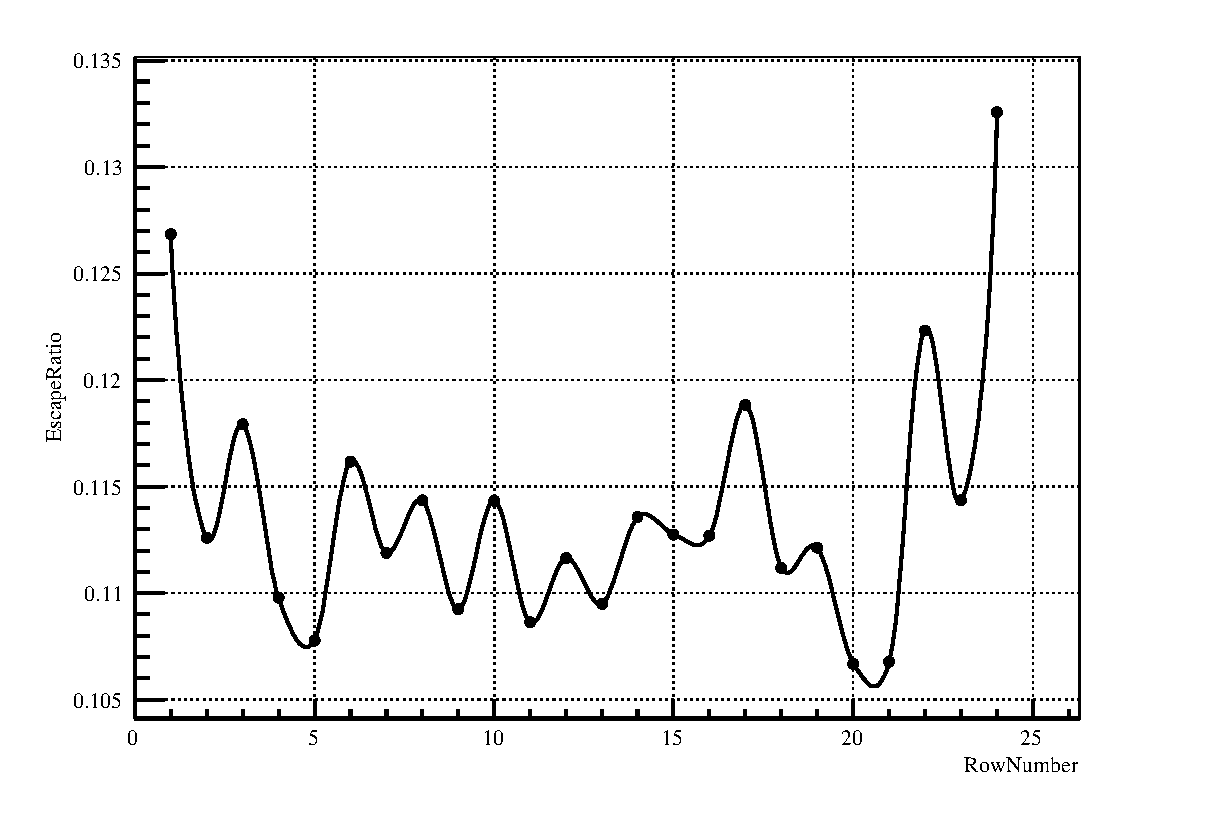
\includegraphics[width=\textwidth]{EscapeRatioNhits1.eps}
  %    \caption{\qihao 每一行泄漏的能量}
  %  \end{figure}
  %\end{frame}
%=========================================
  \section{电子轰击钨靶}
  \begin{frame}\frametitle{200keV电子轰击钨靶}
    \begin{minipage}[t]{0.2\textwidth}
      \liuhao
      右图是动能为$200keV$的电子打到钨靶上,电子沉积能量的位置分布,钨靶边缘的坐标为$-205mm$,这里只
      画了x方向的分布,即电子的入射深度。事例数为$10^7$,一个电子平均要碰撞30多次才能损失掉所有
      能量。
    \end{minipage}
    \begin{minipage}[t]{0.8\textwidth}
      \begin{figure}[ht]
	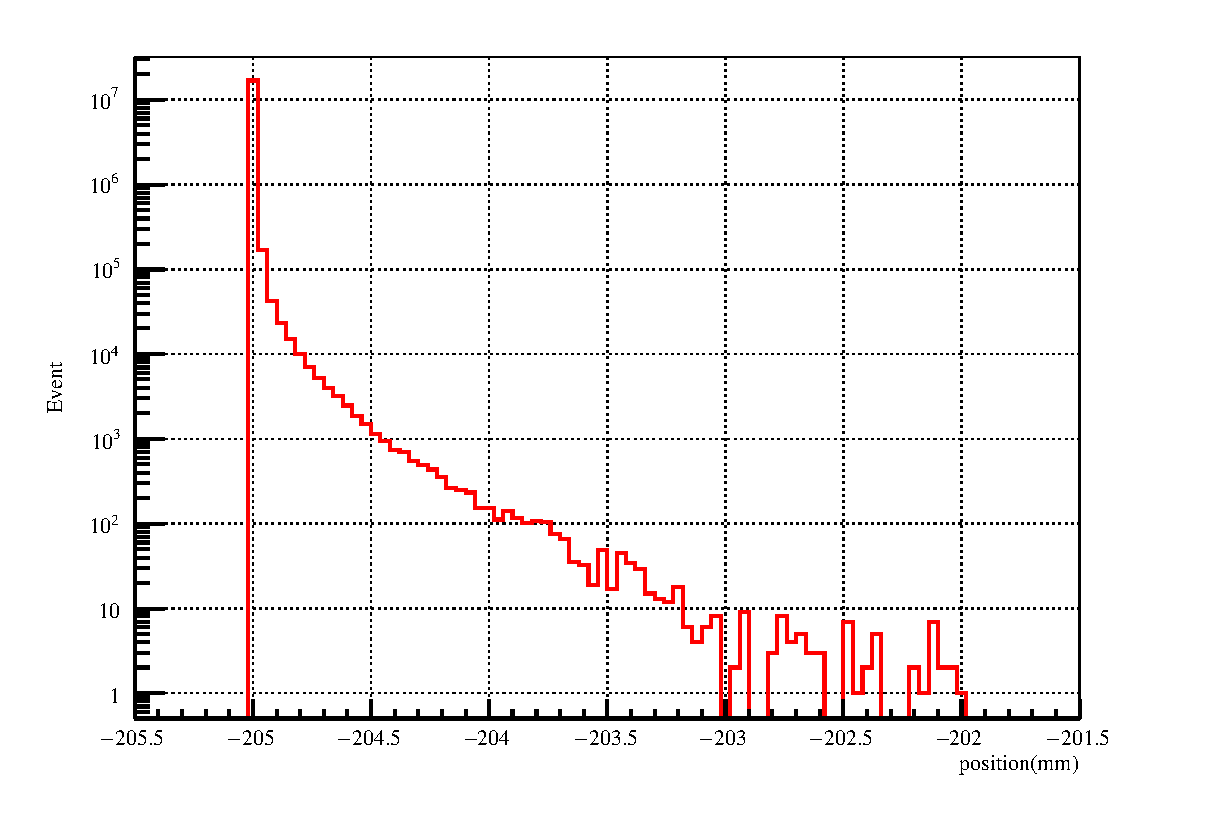
\includegraphics[width=\textwidth]{depositPosition.eps}
	\caption{\qihao 电子入射深度置分布}
      \end{figure}
    \end{minipage}
  \end{frame}
  %===================
  \begin{frame}\frametitle{电子入射深度}
    \begin{figure}[ht]
      \includegraphics[width=\textwidth]{depositPositionRatio.png}
      \caption{\qihao 电子入射深度}
    \end{figure}
  \end{frame}
  %============================
  \section{铅+聚乙烯对射线的屏蔽}
  \begin{frame}\frametitle{铅的衰减系数}
    \begin{itemize}
      \item \liuhao 在模拟过程中发现拟合的衰减系数跟网上的数据不一样。
    \end{itemize}
    \begin{figure}[ht]
      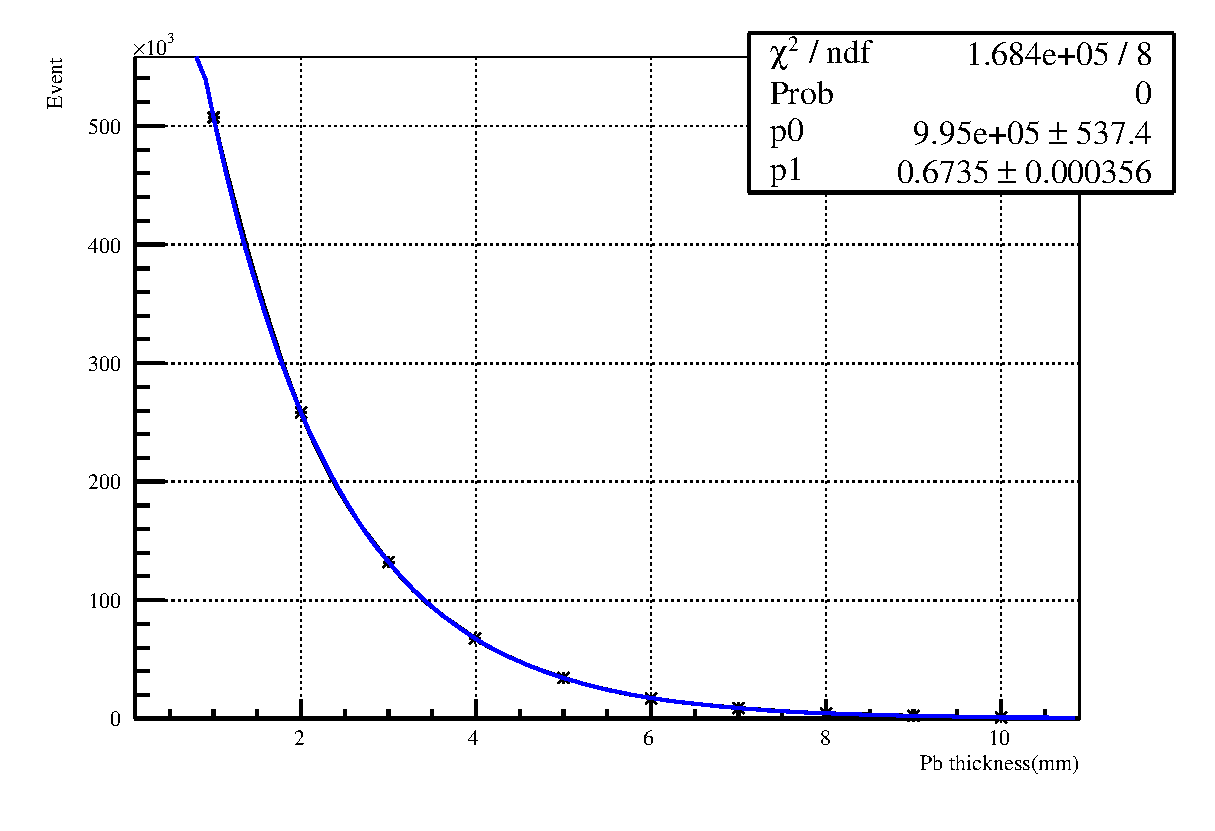
\includegraphics[width=0.33\textwidth]{matPb250kevGammaMu.eps}
      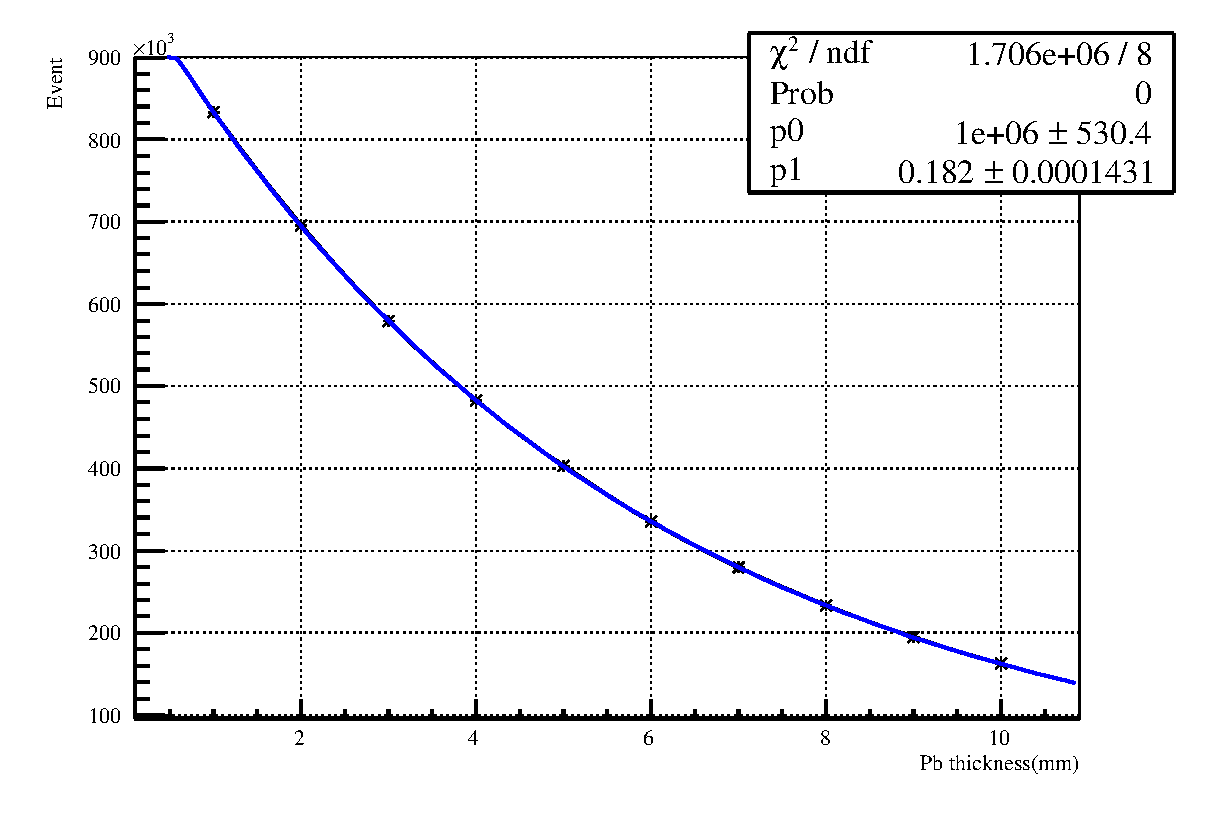
\includegraphics[width=0.33\textwidth]{matPb500kevGammaMu.eps}
      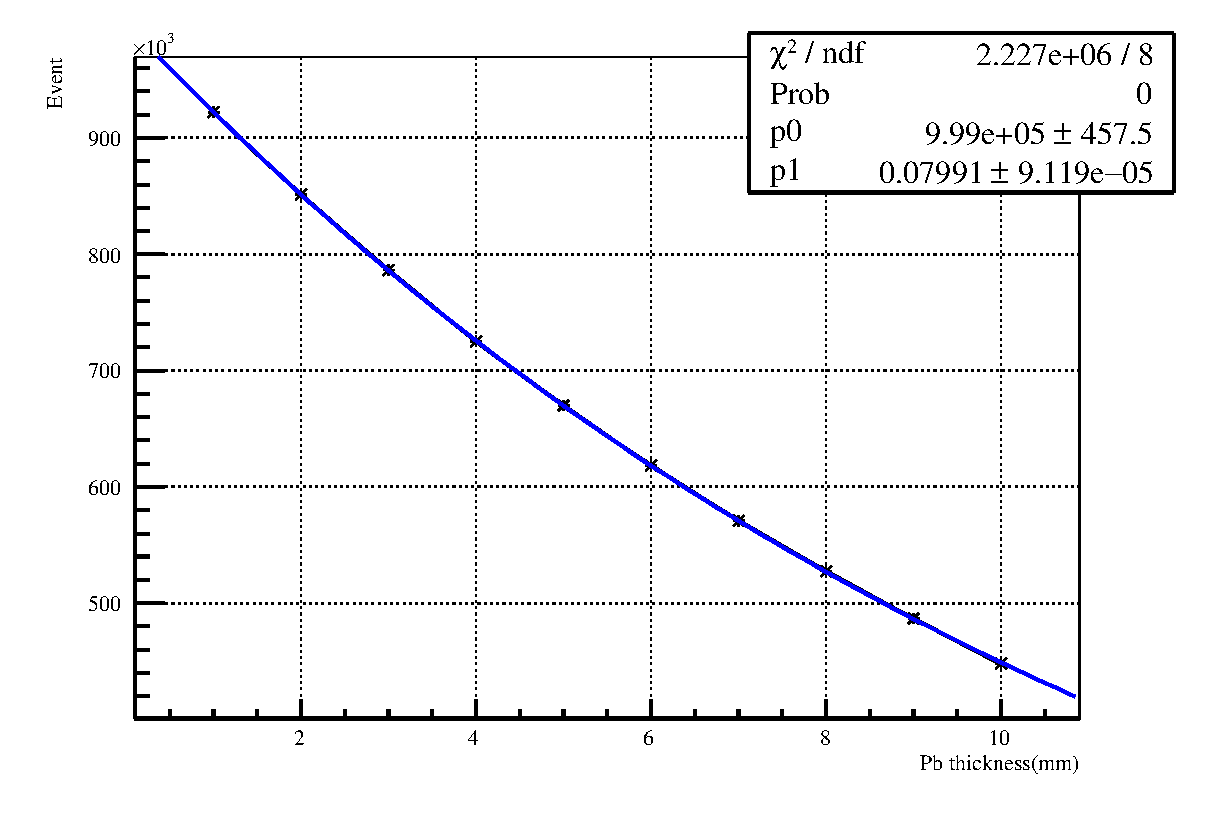
\includegraphics[width=0.33\textwidth]{matPb1MevGammaMu.eps}
      
      \includegraphics[width=0.33\textwidth]{matPb1500kevGammaMu.eps}
      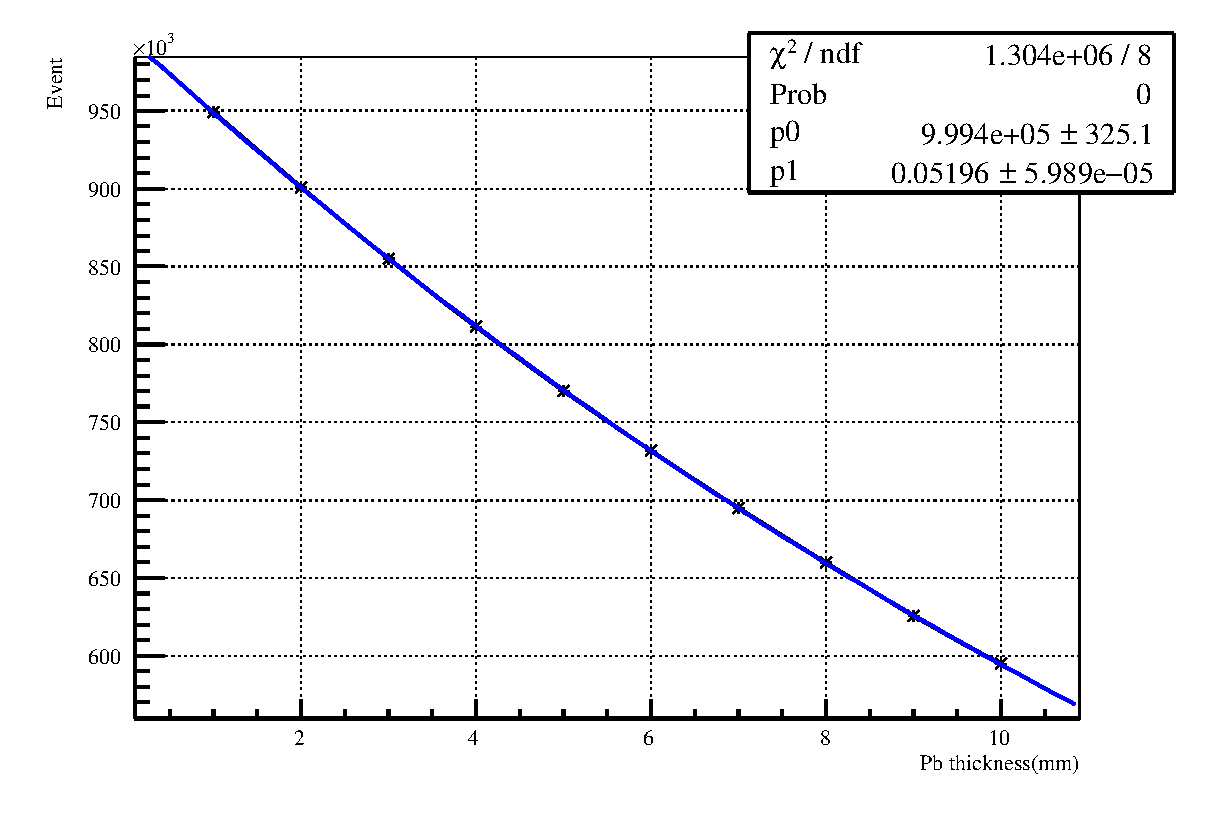
\includegraphics[width=0.33\textwidth]{matPb2MevGammaMu.eps}
      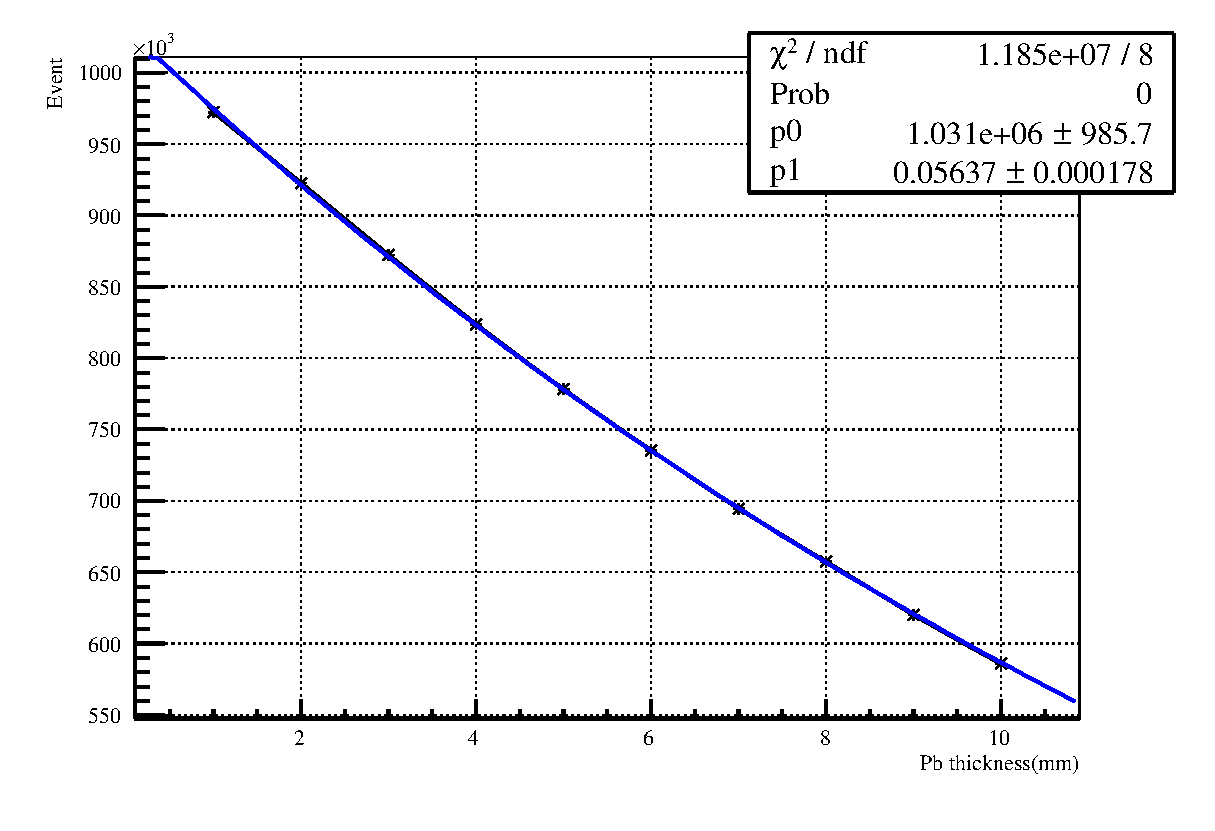
\includegraphics[width=0.33\textwidth]{matPb10MevGammaMu.eps}
    \end{figure}
  \end{frame}
  %============================
  \begin{frame}\frametitle{聚乙烯+铅屏蔽层}
    \begin{minipage}[t]{0.25\textwidth}
      \liuhao
      模拟射线穿过$40mm$的聚乙烯和$5mm$的铅层,透射(1,2,3)、反射(4)及死在屏蔽层(5,6)的光子的
      数目和能量,右图为各部分的能谱,如果只把3看做透射,则其
      比例为$2\times 10^{-5}$。

      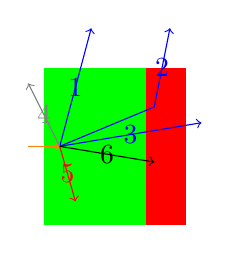
\begin{tikzpicture}
	\fill[green] (0.2,-1) rectangle (1.5,1);
	\fill[red] (1.5,-1) rectangle (2,1);
	\draw[color=orange][->] (0,0)--(0.4,0);
	\draw[color=blue][->] (0.4,0) to node{1} (0.8,1.5);
	\draw[color=blue][->] (0.4,0) to node{3} (2.2,0.3);
	\draw[color=blue][->] (0.4,0)--(1.6,0.5) to node{2} (1.8,1.5);
	\draw[color=gray][->] (0.4,0) to node{4} (0,0.8);
	\draw[color=red][->] (0.4,0) to node{5} (0.6,-0.7);
	\draw[color=black][->] (0.4,0) to node{6} (1.6,-0.2);
      \end{tikzpicture}
    \end{minipage}
    \begin{minipage}[t]{0.7\textwidth}
      \vskip -0.2cm
      \begin{figure}
	\centering
	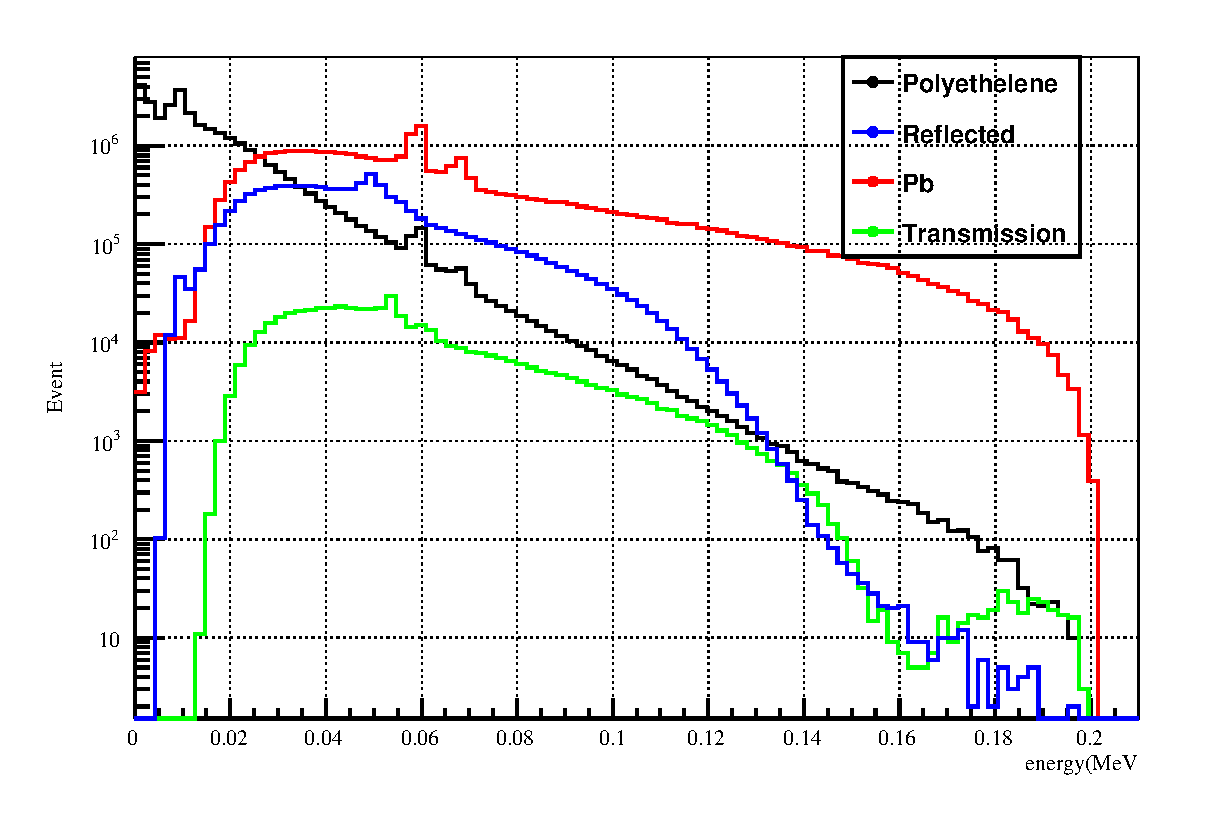
\includegraphics[width=\textwidth]{Spectrum.eps}
      \end{figure}
      \vskip -0.8cm
      \begin{table}
	\liuhao
	总事例数为$5\times 10^8$。

	\qihao
	\begin{tabular}{ c!{\vrule} c c c c }
	  \hline
	             &反射   &透射   &聚乙烯  &铅  \\
	  \hline
	  能量($MeV$)&424715 &28308.5&459582  &$1.737\times 10^6$\\
	  数目       &9127588&517075 &12312964&28042373 \\
	\end{tabular}
      \end{table}
    \end{minipage}
  \end{frame}
  \ThankYouPage
\end{CJK*}
\end{document}
